\chapter{Mask R-CNN}
\label{chap:maskrcnn}

In this chapter, the Mask R-CNN or Mask Region-based Convolutional Neural Network is introduced as a framework to be used to overcome the Airbus ship detection challenge.  Based on the defined classes or objects, the system detects the objects and delivers their respective masks. The image segmentation property of this framework makes it a powerful tool for the ship detection challenge. In this section, the background of the model is explored first. Afterward, the model itself together with its components will be introduced. How this model handles the data, the model and its data delivery will be inspected subsequently.  Finally, the evaluation and improvement suggestion will be provided.

\section{Related Works}
\label{sec:relatedworks}

The computer vision section has improved rapidly in object detection and semantic segmentation thanks to the baseline systems, such as Fast R-CNN \cite{Girshick15}, Faster R-CNN \cite{RenHG015} and Fully Convolutional Network (FCN) \cite{LongSD14}. Compared to the mentioned computer vision tasks, the task of image segmentation has proven to be very challenging. Due to the challenging nature of instance segmentation, the development team of the Mask R-CNN has targeted a framework for this task, which is comparable to those mentioned earlier in performance, robustness and flexibility \cite{HeGDG17}. Before diving into the framework and its components, the image segmentation and R-CNN or Region-based CNN will be explored for setting the ground of the Mask R-CNN.

\subsection{R-CNN and paving the way towards the Mask R-CNN}
\label{subsec:imagesegmentation}

The Region-based Convolutional Neural Network approach generates category-independent region proposals, called Region of Interests or RoI, by using a region proposal module. Each region is then fed individually to a CNN (part of a large CNN) which acts as a feature extraction component. The CNN extracts a fixed-length vector from each region and produces feature vectors as output, which is also fed to set of SVMs \footnote{Support Vector Machine} for classification. In other words, it trains the backbone convolutional networks separately (and end-to-end) on every single RoI to classify each RoI into object(s) of interest or background. R-CNN acts mainly as a classifier and make no prediction about object bounds \cite{GirshickDDM13}.

\begin{figure}[h!]
  \centering
  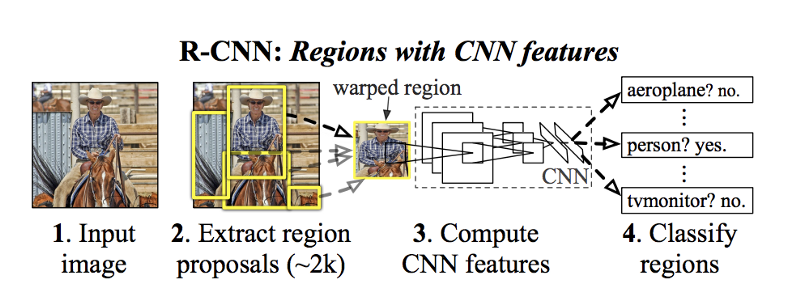
\includegraphics[width=\textwidth]{rcnn}
  \caption[R-CNN]
   {R-CNN Framwork \cite{GirshickDDM13}}
   \label{fig:rcnn}
\end{figure}
\noindent
This method was further improved to enable the attending of RoIs on feature maps by utilizing the RoI Pool, which led to a better performance and accuracy, hence the name Fast R-CNN. In Fast R-CNN, the input of the system is an entire image and a set of object proposals or RoIs. This input is processed by a large CNN together with a max pooling layer. This process pools each RoI into a fixed-sized (convolutional) feature map (containing only RoIs). By using a RoI pooling layer and a sequence of fully connected layers, each RoI on the feature map is then mapped onto a fixed-length feature vector. Finally, a softmax layer predict the class of proposed region and the offset values for the bounding box \cite{Girshick15}.

\begin{figure}[h!]
  \centering
  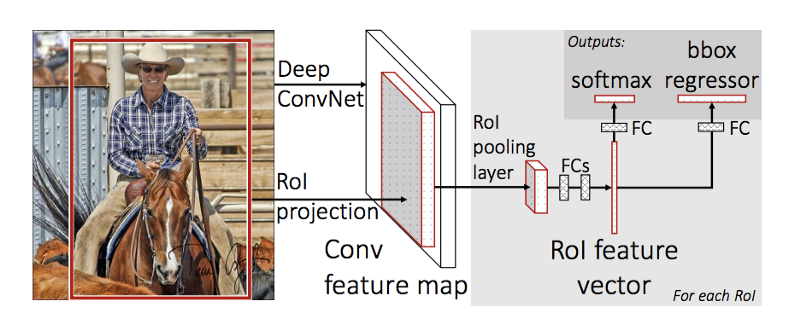
\includegraphics[width=\textwidth, height=5cm]{fast_rcnn}
  \caption[Fast R-CNN]
   {Fast R-CNN Framwork \cite{Girshick15}}
   \label{fig:fast-rcnn}
\end{figure}

\newpage
\noindent
The both mentioned methods uses selective search to generate region proposals, which is a time-consuming task. The Faster R-CNN speeds up the whole process by omitting the selective search algorithm and letting the network learn the region proposal itself. In Faster R-CNN, the system is comprised of a deep fully convolutional network which serves as region proposal module and a Fast R-CNN detector. In this case, the RPN \footnote{Region-based Proposal Network} module  ( utilizing the attention mechanism \cite{ChorowskiBSCB15})  point the regions out to Fast R-CNN module. The RPN module uses sliding-window method and scans over the convolutional feature map, which is generated by the last shared convolutional layer. Multiple region proposals are predicted at the location of each sliding-window which are called anchors. Each anchor (region proposal) is provided with a score that estimates the probability of object or not object \cite{RenHG015}.

\begin{figure}[h!]
  \centering
  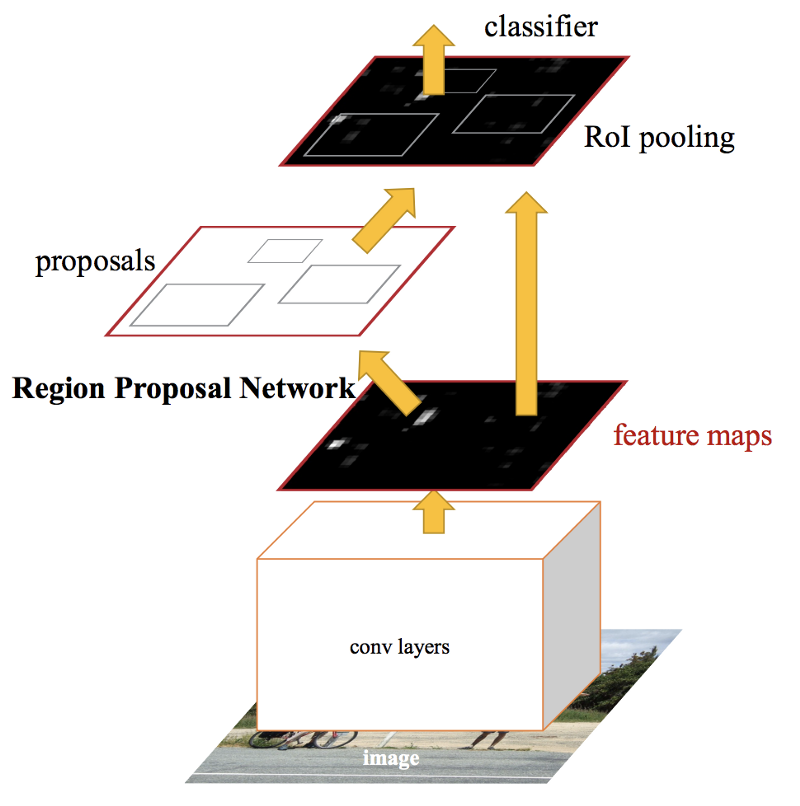
\includegraphics[scale=0.30]{faster_rcnn}
  \caption[Faster R-CNN]
   {Faster R-CNN Framwork \cite{RenHG015}}
   \label{fig:faster-rcnn}
\end{figure}


\subsection{Image Segmentation}
\label{subsec:imagesegmentation}
\noindent
Image segmentation is the process of dividing a digital image into multiple regions or segments, which correspond to different objects or parts of objects. Every pixel in the image is assigned a label which correspond to an object or a class. As a result, a set of pixels, which are labeled identically, shares a specific character. This provides a mean to represent a digital image into a much more meaningful and easier to analyze object \cite{kale2010computer}. 

\begin{figure}[t]
  \centering
  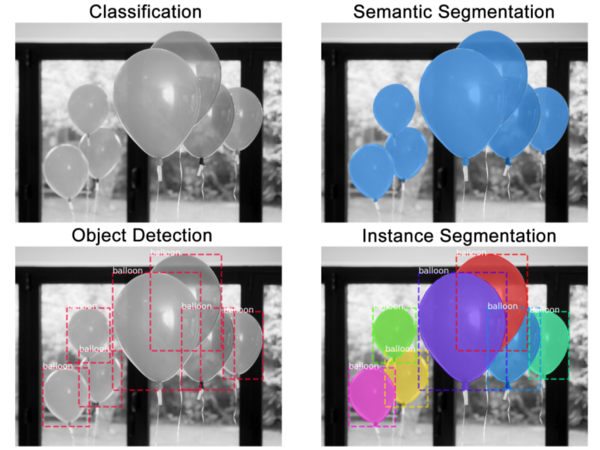
\includegraphics[scale=0.50]{image_segmentation}
  \caption[Image Segmentation]
   {Tasks of Computer Vision  \cite{imgseg}}
   \label{fig:faster-rcnn}
\end{figure}


\section{Mask R-CNN Details}
\label{sec:maskrcnn-details}

The Mask Region-based Convolutional Neural Network adopts the two-stages procedure of Fast R-CNN. It keeps the RPN stage untouched but adds a branch in parallel to the class amd boundary box prediction in second stage, which outputs a binary mask for each RoI\cite{HeGDG17}. The Mask R-CNN framework, which is used for ship detection during this project, was introduced by Kaiming et al., 2017 in Mask R-CNN paper. The Faster R-CNN was the work of the same author who has extended his own framework by developing the Mask R-CNN. 

\begin{figure}[h!]
  \centering
  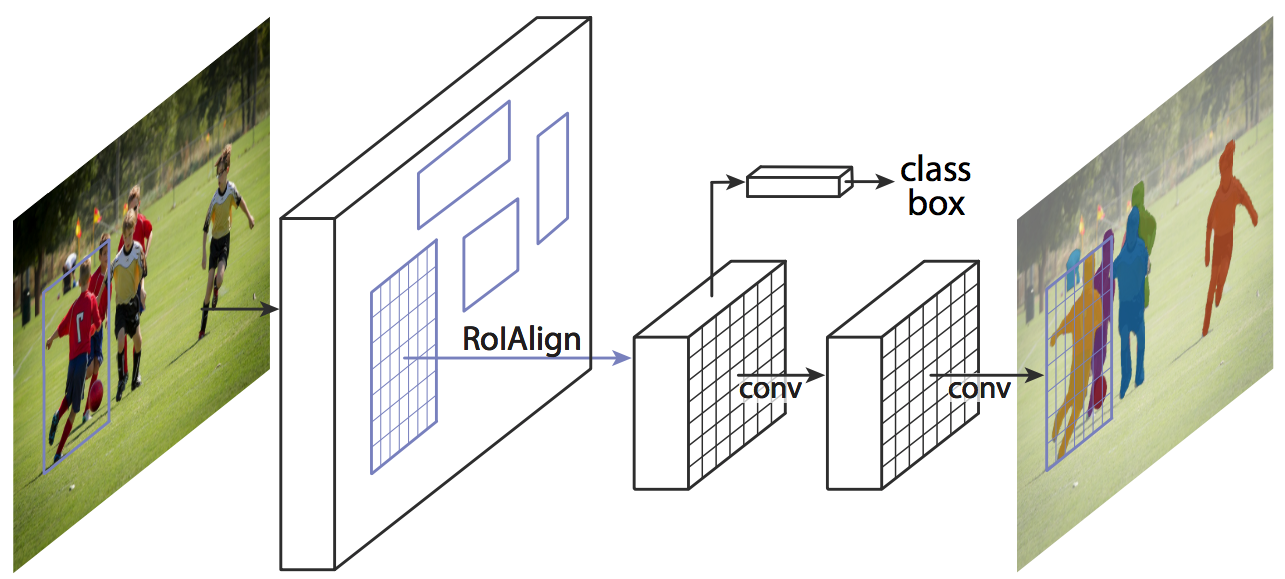
\includegraphics[scale=0.30]{maskrcnn_framework}
  \caption[Mask R-CNN]
   {Mask R-CNN Framwork \cite{HeGDG17}}
   \label{fig:faster-rcnn}
\end{figure}
\noindent
The implementation of the framework is provided by Waleed A. via his Github page \cite{matterport_maskrcnn_2017}. Based on the information provided on his GIthub page, the author has improved the Mask R-CNN on some points. This framework consists of the following components:


\subsection{Backbone}
\label{subsec:backbone}

Backbone which is composed originally of a standard ResNet50 or Resnet101. The backbone is further improved by adding a Feature Pyramid Network(FPN)\footnote{the FPN was also introduced by the author of the Mask R-CNN paper \cite{ LinDGHHB16}}. By Adding this layer, the author seeks a better feature extraction. Diving deeper into this topic is beyond the scope of this project. (image of fpn with cite). The FPN is initiated inside the method \textbf{\textit{MaskRCNN.build()}}

\subsection{RPN}
\label{subsec:rpn}

Region Proposal Network which acts identical to the RPN of Faster R-CNN (see the R-CNN section) ~\ref{subsec:imagesegmentation}. It slides a small network over the generated convolutional feature map and produces anchors at each sliding-window. At this point, the RPN generates two outputs for each anchor, Anchor Class and Bounding Box Refinement. Anchor class indicates one of two classes, either foreground(FG) or background(BG). The foreground class implies that it is likely that this box includes an object.  The Bounding Box Refinement is a foreground anchor, also called positive anchor. This anchor might not be perfectly aligned on the object, therefore the RPN calculates a delta to refine the anchor box, hence the name. The RPN is created in the method \textbf{\textit{rpn\_graph()}} and anchor scales and aspect ratio are governed by two global variables \textbf{\textit{RPN\_ANCHOR\_SCALES}} and \textbf{\textit{RPN\_ANCHOR\_RATIOS}}  located in config file \textbf{\textit{config.py}}. the top anchor which is more likely to contain the object is picked and refined. If there are multiple overlapping anchors, the anchor with highest foreground score will be picked and rest will be discarded.\footnote{Each anchor has a score which is predicted by RPN}. For this purpose, \textbf{\textit{ProposalLayer}}, a custom \textit{Keras layer}, is used. This layer reads the output of RPN, chooses the top/best anchor and applies the bounding box refinement. 

\subsection{RoI Classifier and Bounding Box Regression}
\label{subsec:roi-classifier}

This layer runs over the RoIs generated by RPN from last layer and outputs two properties for each RoI. Class and Bounding Box Refinement. In contrast to RPN layer, this network is deeper and has the ability to map the regions onto specific classes (based on the model, person, chair, ship, cars, animal etc.) Additionally, it generates a background class, which signals the disposal of the RoI. The refinement property is identical to the one of the previous layer. This component is created via the method \textbf{\textit{fpn\_classifier\_graph()}}.

\subsection{RoI Pooling}
\label{subsec:roi-pooling}

Because classifiers are not very capable of handling the inputs with variable sizes, there is a problem needs to be addressed first. The application of Bounding Box Refinement in the RPN section generate RoI boxes of variable sizes. This side effect can be mitigated by RoI Pooling. RoI Pooling refers to cropping and resizing the corresponding part of the convolutional feature map to a   fixed size. \textbf{\textit{ROIAlign}} is the method which is proposed by Kaiming et al., 2017 in Mask R-CNN paper. They sample the feature map at multiple points and apply a bilinear interpolation. This Mask R-CNN, used for this project, implements the \textbf{\textit{ROIAlign}} method via Tensorflow’s \textbf{\textit{crop\_and\_resize}} function, which is simple and delivers very good results (close to the one of the original implementation). ROI pooling is implemented in the class \textbf{\textit{PyramidROIAlign}}.

\subsection{Segmentation Masks}
\label{subsec:seg-mask}

this is the component which makes Mask R-CNN distinguishable from Faster R-CNN. This branch is a convolutional network which generates the binary mask for each (positive) RoI, which were selected by RoI classifier. These are 28x28, low resolution and soft masks. This helps to keep the mask branch light-weighted. During the training, the masks are down-scaled to 28x28 to compute the loss, and during the inferencing, the low-resolution, predicted mask are up-scaled to the size of the bounding box of the RoI. This will give us the final mask (one per object). The mask branch is implemented in the method \textbf{\textit{build\_fpn\_mask\_graph()}}.

\section{Ship Data Inspection}
\label{sec:shipdata}

\textbf{Loading confi}
\begin{lstlisting}
#ship data
config = ship.ShipConfig()
SHIP_DIR = TRAIN_DATA_DIR
\end{lstlisting}

\textbf{Dataset}
\begin{lstlisting}
train_dataset_filenames = data_utils.load_filenames(SHIP_DIR)
# make sure that the filenames have a fixed order before shuffling
train_dataset_filenames.sort() 
np.random.seed(230)
# shuffles the ordering of filenames (deterministic given the chosen seed)
np.random.shuffle(train_dataset_filenames) 
train_len = int(0.3*len(train_dataset_filenames))
valid_len = len(train_dataset_filenames) - train_len
dataset_train_filenames = train_dataset_filenames[:train_len]
dataset_val_filenames = train_dataset_filenames[train_len:]
# Load dataset
dataset = ship.ShipDataset()
dataset.filenames.extend(dataset_train_filenames)
dataset.load_ship(SHIP_DIR)
dataset.prepare()
\end{lstlisting}

\textbf{Display Samples}
\begin{lstlisting}
# Load and display random samples
image_ids = np.random.choice(dataset.image_ids, 4)
for idx, image_id in enumerate(image_ids):
    image = dataset.load_image(image_id)
    mask, class_ids = dataset.load_mask(image_id)
    visualize.display_top_masks(image, mask, class_ids, dataset.class_names, img_idx=idx)
\end{lstlisting}

\begin{figure}[h!]
  \centering
  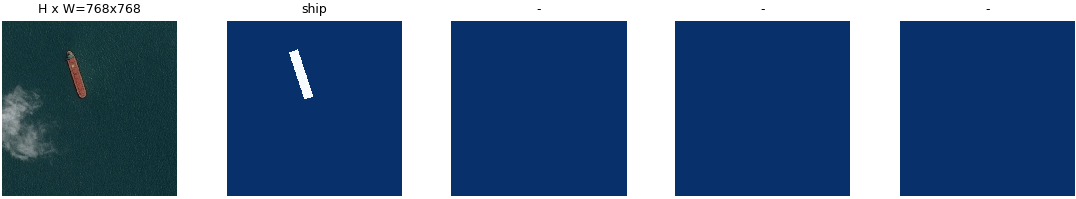
\includegraphics[width=\textwidth]{image_withMasks_0}
  \caption[Random image with mask]
   {Image with mask}
   \label{fig:rndimg}
\end{figure}

\textbf{Bounding Boxes}
\begin{lstlisting}
# Load random image and mask.
for idx, image_id in enumerate(image_ids):
    image = dataset.load_image(image_id)
    mask, class_ids = dataset.load_mask(image_id)
   # Compute Bounding box
    bbox = utils.extract_bboxes(mask)
    # Display image and additional stats
    print("image_id ", image_id, dataset.image_reference(image_id))
    log("image", image)
    log("mask", mask)
    log("class_ids", class_ids)
    log("bbox", bbox)
    # Display image and instances
    visualize.display_instances(image, bbox, mask, class_ids, dataset.class_names, img_idx=idx)
\end{lstlisting}

\begin{figure}[h!]
  \centering
  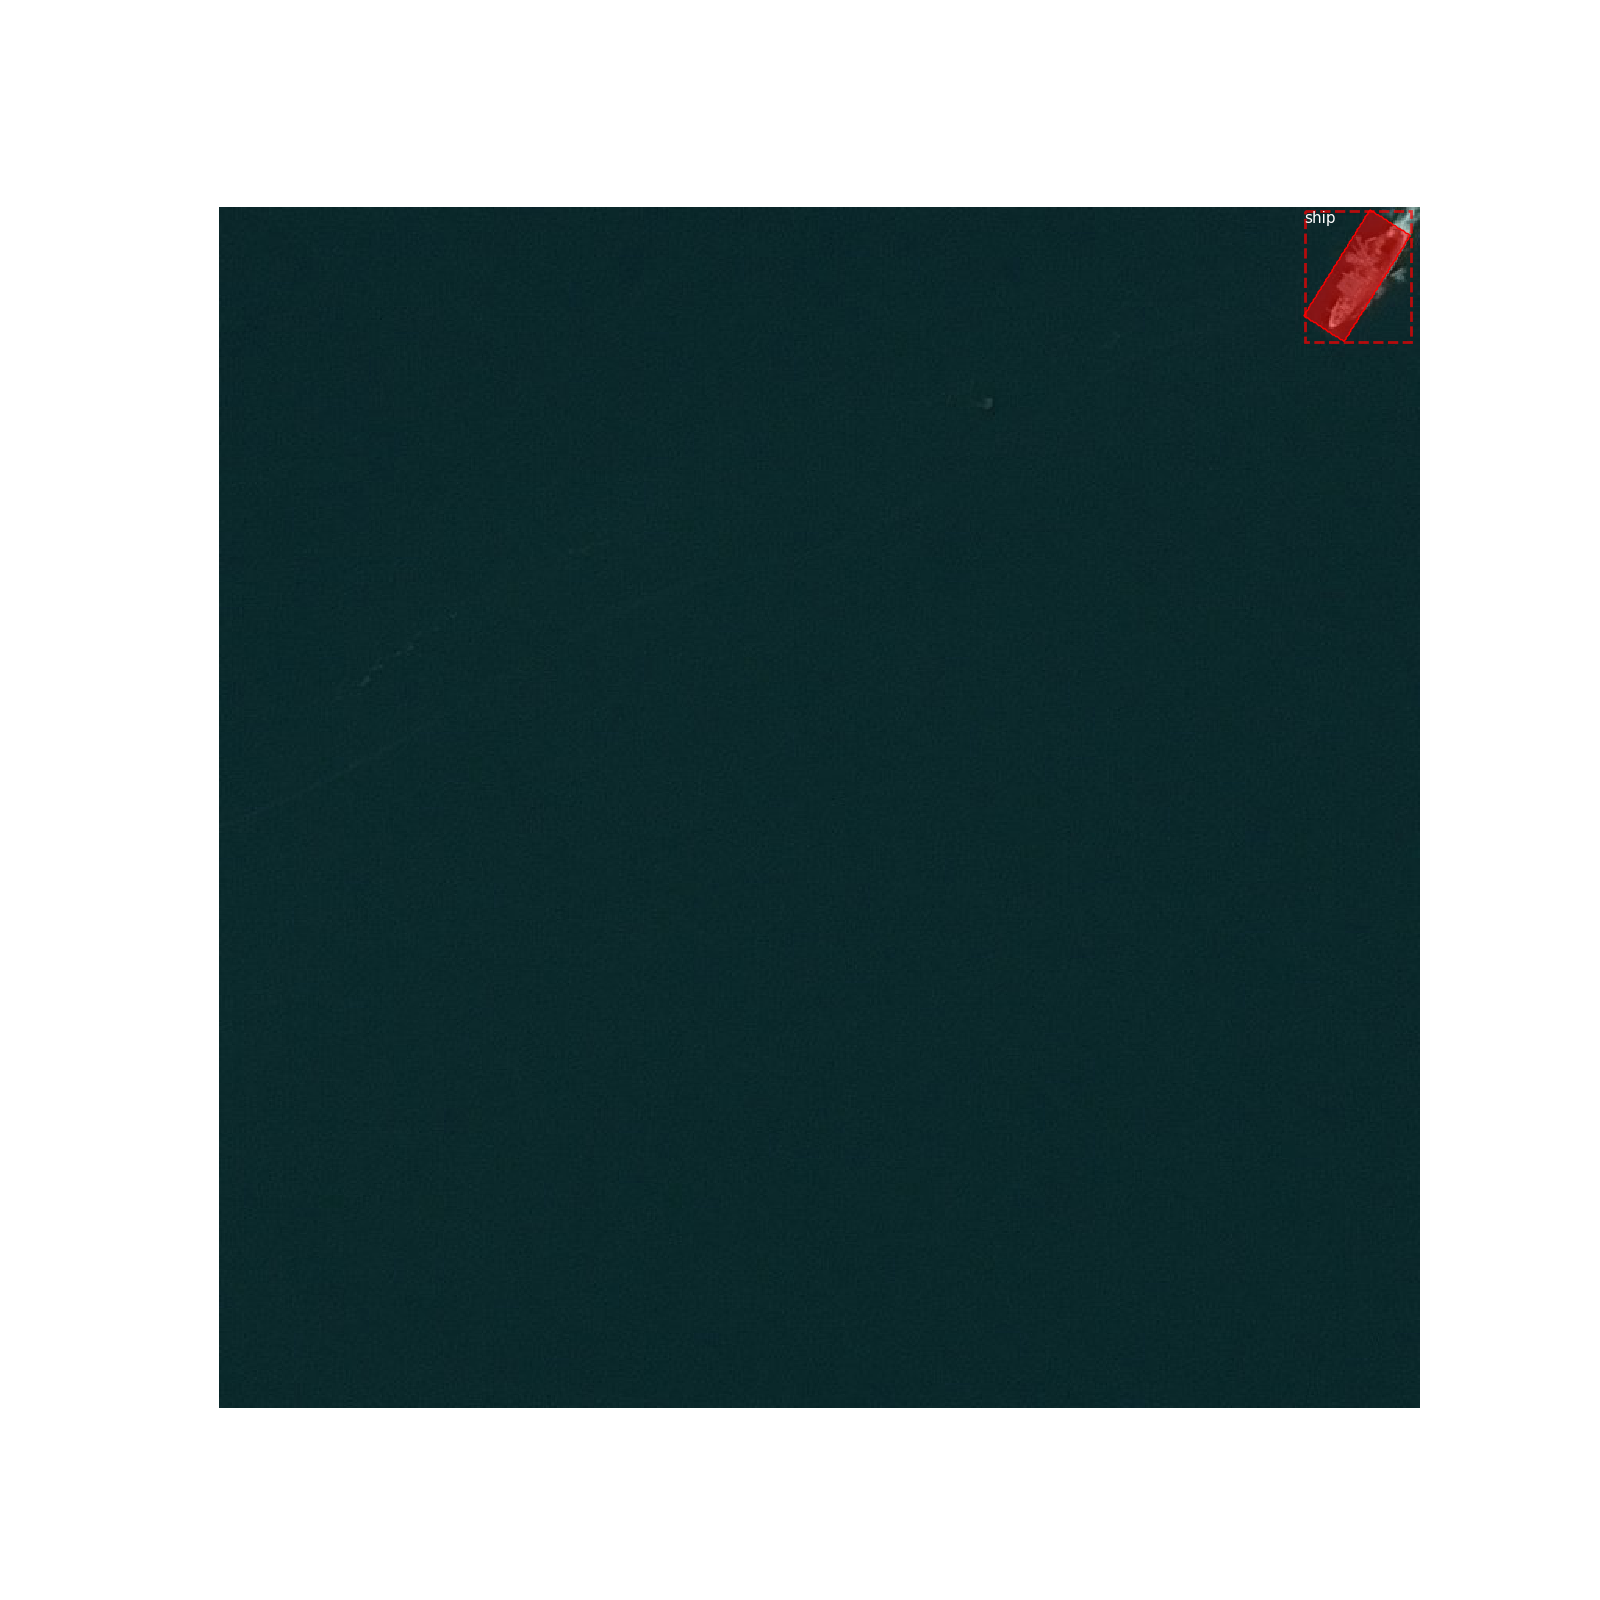
\includegraphics[width=\textwidth]{img_0_with_bounding_box}
  \caption[Random image with bounding box]
   {Image with bounding box}
   \label{fig:imgbbx}
\end{figure}

\newpage
\textbf{Positive Anchors}
\begin{lstlisting}
b = 0
# Restore original image (reverse normalization)
sample_image = modellib.unmold_image(normalized_images[b], config)
# Compute anchor shifts.
indices = np.where(rpn_match[b] == 1)[0]
refined_anchors = utils.apply_box_deltas(anchors[indices], rpn_bbox[b, :len(indices)] * config.RPN_BBOX_STD_DEV)
log("anchors", anchors)
log("refined_anchors", refined_anchors)
# Get list of positive anchors
positive_anchor_ids = np.where(rpn_match[b] == 1)[0]
print("Positive anchors: {}".format(len(positive_anchor_ids)))
negative_anchor_ids = np.where(rpn_match[b] == -1)[0]
print("Negative anchors: {}".format(len(negative_anchor_ids)))
neutral_anchor_ids = np.where(rpn_match[b] == 0)[0]
print("Neutral anchors: {}".format(len(neutral_anchor_ids)))
# ROI breakdown by class
for c, n in zip(dataset.class_names, np.bincount(mrcnn_class_ids[b].flatten())):
    if n:
        print("{:23}: {}".format(c[:20], n))
# Show positive anchors
fig, ax = plt.subplots(1, figsize=(16, 16))
visualize.draw_boxes(sample_image, boxes=anchors[positive_anchor_ids], 
                     refined_boxes=refined_anchors, ax=ax)
\end{lstlisting}

\begin{figure}[h!]
  \centering
  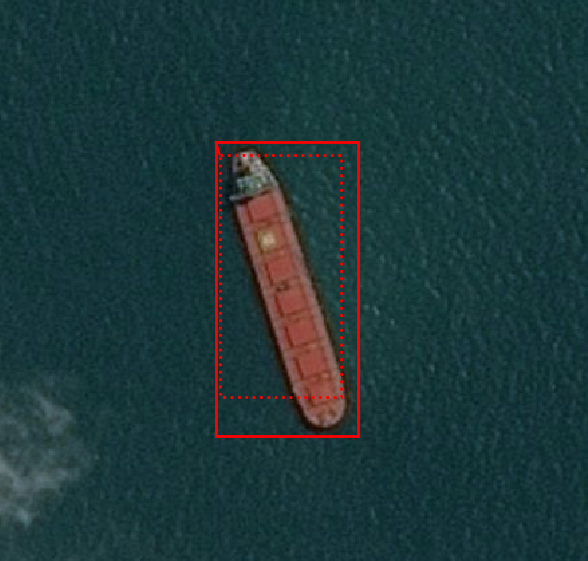
\includegraphics[width=\textwidth]{pos_ancher_img}
  \caption[Image with positive anchors]
   {Image with positive anchors}
   \label{fig:posanchors}
\end{figure}

\textbf{Negative Anchores}
\begin{lstlisting}
# Show negative anchors
visualize.draw_boxes(sample_image, boxes=anchors[negative_anchor_ids])
\end{lstlisting}
\begin{figure}[t]
  \centering
  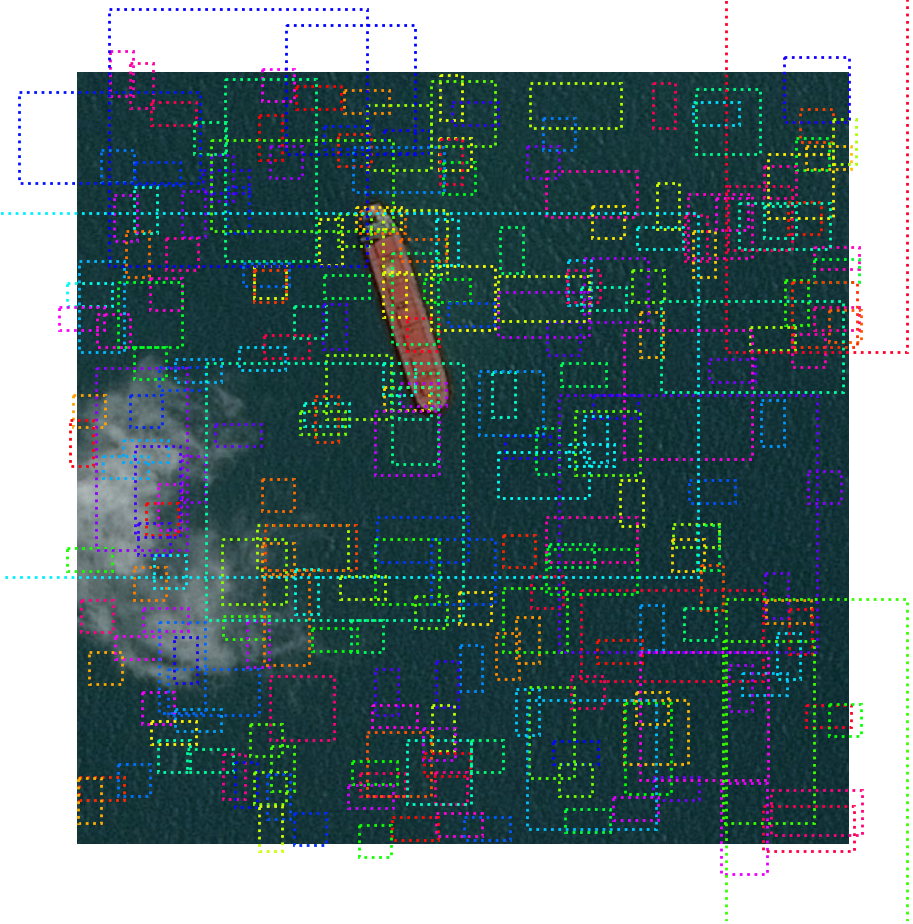
\includegraphics[width=\textwidth]{image_negative_anchors_1}
  \caption[Image with negative anchors]
   {Image with negative anchors}
   \label{fig:neganchors}
\end{figure}

\newpage
\textbf{RoIs}
\begin{lstlisting}
if random_rois:
    # Class aware bboxes
    bbox_specific = mrcnn_bbox[b, np.arange(mrcnn_bbox.shape[1]), mrcnn_class_ids[b], :]

    # Refined ROIs
    refined_rois = utils.apply_box_deltas(rois[b].astype(np.float32), bbox_specific[:,:4] * config.BBOX_STD_DEV)

    # Class aware masks
    mask_specific = mrcnn_mask[b, np.arange(mrcnn_mask.shape[1]), :, :, mrcnn_class_ids[b]]

    visualize.draw_rois(sample_image, rois[b], refined_rois, mask_specific, mrcnn_class_ids[b], dataset.class_names)
    
    # Any repeated ROIs?
    rows = np.ascontiguousarray(rois[b]).view(np.dtype((np.void, rois.dtype.itemsize * rois.shape[-1])))
    _, idx = np.unique(rows, return_index=True)
    print("Unique ROIs: {} out of {}".format(len(idx), rois.shape[1]))
\end{lstlisting}

\begin{figure}[h!]
  \centering
  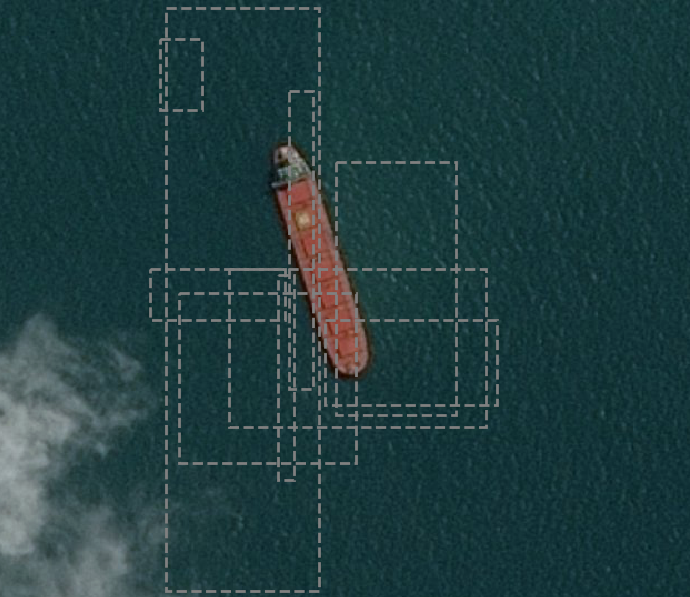
\includegraphics[width=\textwidth]{all_random_rois_img}
  \caption[Image with random RoIs]
   {Image with random RoIs}
   \label{fig:randomrois}
\end{figure}

\newpage
\section{Trained Model Inspection}
\label{sec:trainedmodel}







































